\subsubsection{Genotypes and Genotyping} \label{background:biology:genotype_and_genotyping}
Much like variant, the term \textit{genotype} is used slightly ambiguously in the world of bioinformatics. 
The term genotype may be used to refer to an individual's total genetic makeup.
It may also be used to refer to the variants an individual carries in its chromosomes at a particular location along the genome.
Throughout this thesis, we assume the latter definition.
For humans, who have two copies of each chromosome, we may have the same or two different variations present at a particular location in the genome, making up the genotype.

\textit{Genotyping} an individual refers to the process of determining which genotypes an individual carries. 
For humans, this would entail determining the set of variants present at each variant site.
In most genotyping software tools today, genotypes are given in a format that specifies whether a particular variant is present in none, one or both of a human's chromosomes.
For instance, given a reference genome sequence where a variant site is known to could manifest an A at a particular allele where the reference sequence contains a G, a human individual's genotype for this variant could either be referred to as $0/0$, meaning that the variant allele A is present in neither of the chromosomes, $0/1$, meaning that it is present in one of the chromosomes, or $1/1$, meaning that it is present in both chromosomes.

\definecolor{variantcolor}{RGB}{235,235,235}

\begin{figure}[H]
\begin{center}
\scalebox{0.85}{
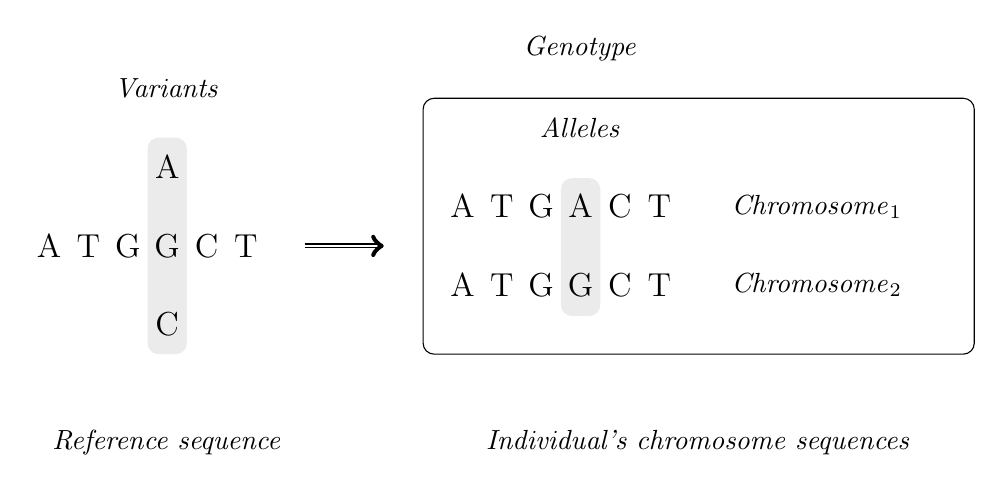
\begin{tikzpicture}
  % Variants
  \node at(2.25,2)(title){\textit{Variants}};
  \node at(2.25,0)[rounded corners,minimum width=0.5cm,minimum height=2.75cm, fill=variantcolor](variant){};
  % Sequence (left)
  \node at(0.75,0)(n2){\large A};
  \node at(1.25,0)(n3){\large T};
  \node at(1.75,0)(n4){\large G};
  \node at(2.25,1)(n5){\large A};
  \node at(2.25,0)(n5){\large G};
  \node at(2.25,-1)(n5){\large C};
  \node at(2.75,0)(n5){\large C};
  \node at(3.25,0)(n5){\large T};
  % Arrow
  %\draw [-stealth](4,0) -- (5,0);
  %\draw [thick,->](4,0) -- (5,0);
  \draw [double distance=1pt,->](4,0) -- (5,0);
  % Genotype
  \node at(7.5,2.5)(title){\textit{Genotype}};
  \node at(9,0.25)[rectangle,rounded corners,draw,minimum width=7cm,minimum height=3.25cm](genotype){};
  % Alleles 
  \node at(7.5,1.5)(title){\textit{Alleles}};
  % Chromosomes
  \node at(10.5,0.5)(title){\textit{Chromosome}$_1$};
  \node at(10.5,-0.5)(title){\textit{Chromosome}$_2$};
  \node at(7.5,-.015)[rounded corners,minimum width=0.5cm,minimum height=1.75cm, fill=variantcolor](variant){};
  % Chromosome 1 sequence
  \node at(6,0.5)(n2){\large A};
  \node at(6.5,0.5)(n3){\large T};
  \node at(7,0.5)(n4){\large G};
  \node at(7.5,0.5)(n5){\large A};
  \node at(8,0.5)(n5){\large C};
  \node at(8.5,0.5)(n5){\large T};
  % Chromosome 2 sequence
  \node at(6,-0.5)(n2){\large A};
  \node at(6.5,-0.5)(n3){\large T};
  \node at(7,-0.5)(n4){\large G};
  \node at(7.5,-0.5)(n5){\large G};
  \node at(8,-0.5)(n5){\large C};
  \node at(8.5,-0.5)(n5){\large T};
  % Reference and the individual's chromosomes
  \node at(2.25,-2.5)(ref){\textit{Reference sequence}};
  \node at(9,-2.5)(ind){\textit{Individual's chromosome sequences}};
\end{tikzpicture}
}
\caption{
  In humans, who carry two copies of every chromosome, a genotype constitutes a set of two alleles or variants - one in each chromosome at the variant site. 
  Along the reference sequence on the left, several possible variants may be known to occur at a specific site. 
  After examining the sequence of an individual, we try to determine the individual's genotype by scoring which variants are present in each chromosome at the location of interest.
  In this illustration, the individual's genotype may be described as two scores: $0/1$ for the SNP variant where the G is replaced by an A in chromosome$_1$, and $0/1$ for the G remaining the same as in the reference in chromosome$_2$.
}
\label{figure:variant_and_genotype}
\end{center}
\end{figure}

Today, the most established ways to genotype individuals are based on \textit{alignment-based} methods.
Such methods rely on aligning sequenced DNA reads to a reference genome and performing variant calling before calling genotypes by assessing which genotypes are most probable based on locally supported variants \cite{gatk}.
However, given the vast amount of reads provided by high-throughput sequencing technologies today, aligning each read to a $3*10^9$ long reference sequence is very compute, memory and time consuming.
As a result, a set of new prominent methods have emerged in recent years to help alleviate these issues.
\textit{Alignment-free} genotyping methods, where the alignment of reads and variant calling step are skipped altogether, have yielded promising results and significant speedup compared to their alignment-based counterparts.
In such methods, small parts of the sequenced reads called \textit{k}mers are analyzed, and statistical models are used to compute genotype-probabilities supported by the results from the \textit{k}mer analysis and previous knowledge of variants and genotypes that have been accumulated over years of research \cite{kage,malva,1000_genomes_project}.
One such alignment-free genotyper, KAGE, has recently shown that it can genotype a human individual more than 10 times faster than any other known genotyper tool, while still providing competitive accuracy scores for its genotype calls \cite{kage}.

